\chapter{Metodologia}
% ---
% ---
Neste segmento, serão delineadas informações relacionadas à elaboração da aplicação proposta neste projeto. Discutiremos a Estruturação do desenvolvimento, a Análise de requisitos, abrangendo tanto os funcionais quanto os não funcionais.

Para a realização deste trabalho, em termos de sua natureza, foi adotada a metodologia de pesquisa aplicada. Conforme \begin{citacao}
	\cite{fleury2016pesquisa}
	a pesquisa aplicada concentra-se em torno dos problemas presentes nas atividades das instituições, organizações, grupos ou atores sociais. Ela está empenhada na elaboração de 
    diagnósticos, identificação de problemas e busca de soluções
\end{citacao} 

\section{Estruturação do desenvolvimento}
A forma como foi organizado o desenvolvimento do presente trabalho foi dividio em etapas, sendo elas:
\begin{itemize}
	\item Análise de Requisitos
	\item Criação da estrutura para armazenamento de dados
	\item Desenvolvimento da aplicação Web
\end{itemize}

Conforme demonstrado na \autoref{fig:grafico-etapas-desenvolvimento}:

\begin{figure}[htb]
    \caption{\label{fig:grafico-etapas-desenvolvimento}Etapas de Desenvolvimento}
    \begin{center}
        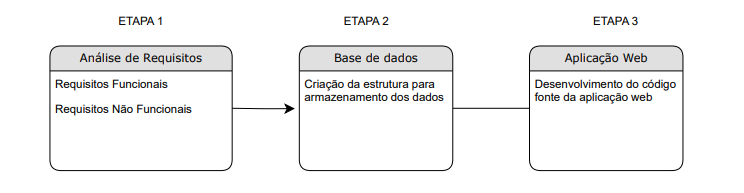
\includegraphics[scale=0.9]{imagens/estagios-de-desenvolvimento.png}
    \end{center}
\end{figure}


\section{Análise de Requisitos}
Os requisitos inerentes a aplicação web AutoForm foram identificados por meio de entrevistas conduzidas com um membro do setor de Tecnologia da Brigada Militar, SD. Tiago Costa. Durante essas entrevistas, foram formuladas perguntas pertinentes ao procedimento de geração do AEL.

A coleta de dados foi complementada por meio da análise de documentos, da portaria 136, mais especificamente o anexo D do \cite{ExércitoBrasileiro} constante nos Anexos (\ref{sec:anexoA1}, \ref{sec:anexoA2}, \ref{sec:anexoA3}, \ref{sec:anexoA4}). Esta documentação conceitua todas as fases envolvidas no processo de geração do AEL da Brigada Militar do Rio Grande do Sul. Nesse contexto, foram examinadas as dificuldades  encontradas pelos operadores na execução desse processo, a fim de determinar as funcionalidades essenciais para o pleno funcionamento da aplicação, quais devem ser implementadas durante o desenvolvimento do sistema. Ademais, foi realizada uma avaliação para determinar as funcionalidades desejáveis.

\subsection{Requisitos Funcionais}
Nesta subseção, será abordado os requisitos funcionais, aqueles que abrangem e descrevem todas as funcionalidades previstas para o sistema. 

\begin{table}[h]
    \caption{Requisito Funcional 1}
    \centering
    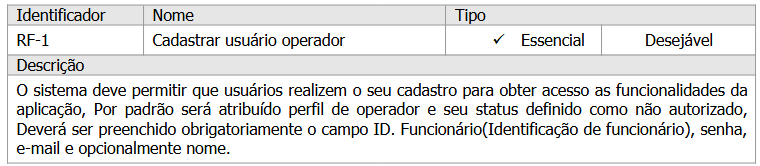
\includegraphics[scale=0.9]{imagens/rf01.png}
    \label{tab:rf01}
    \legend{Fonte: Autor}
\end{table}

\begin{table}[h]
    \caption{Requisito Funcional 2}
    \centering
    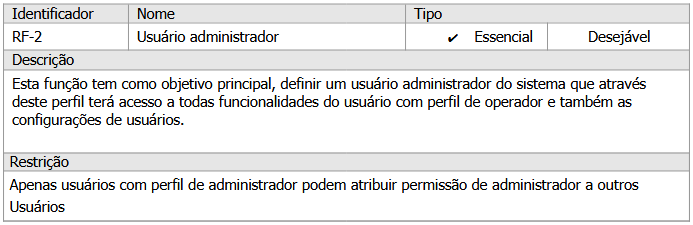
\includegraphics[scale=0.9]{imagens/rf02.png}
    \label{tab:rf02}
    \legend{Fonte: Autor}
\end{table}

\begin{table}[h]
    \caption{Requisito Funcional 3}
    \centering
    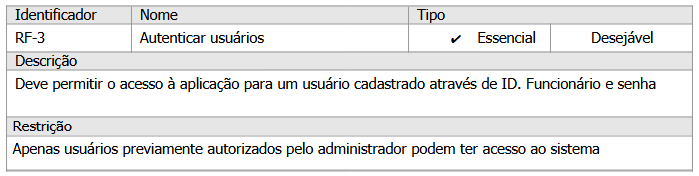
\includegraphics[scale=0.9]{imagens/rf03.png}
    \label{tab:rf03}
    \legend{Fonte: Autor}
\end{table}

\begin{table}[h]
    \caption{Requisito Funcional 4}
    \centering
    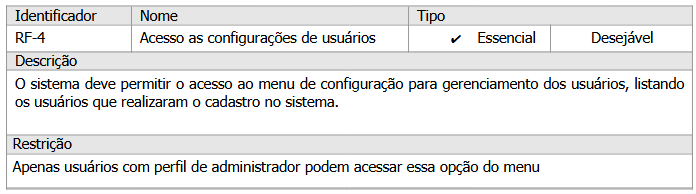
\includegraphics[scale=0.9]{imagens/rf04.png}
    \label{tab:rf04}
    \legend{Fonte: Autor}
\end{table}

\begin{table}[h]
    \caption{Requisito Funcional 5}
    \centering
    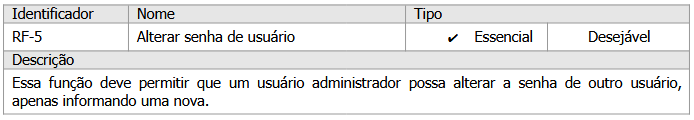
\includegraphics[scale=0.9]{imagens/rf05.png}
    \label{tab:rf05}
    \legend{Fonte: Autor}
\end{table}

\begin{table}[h]
    \caption{Requisito Funcional 6}
    \centering
    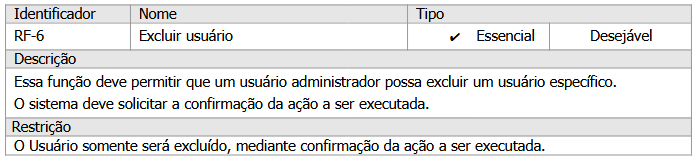
\includegraphics[scale=0.9]{imagens/rf06.png}
    \label{tab:rf06}
    \legend{Fonte: Autor}
\end{table}

\begin{table}[h]
    \caption{Requisito Funcional 7}
    \centering
    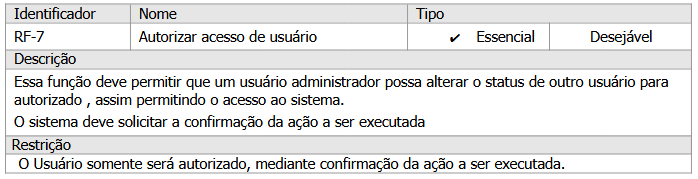
\includegraphics[scale=0.9]{imagens/rf07.png}
    \label{tab:rf07}
    \legend{Fonte: Autor}
\end{table}

\begin{table}[h]
    \caption{Requisito Funcional 8}
    \centering
    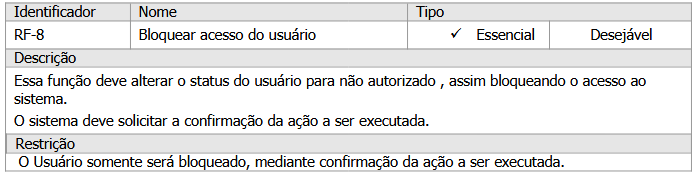
\includegraphics[scale=0.9]{imagens/rf08.png}
    \label{tab:rf08}
    \legend{Fonte: Autor}
\end{table}

\begin{table}[h]
    \caption{Requisito Funcional 9}
    \centering
    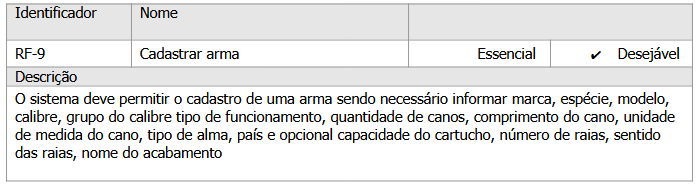
\includegraphics[scale=0.9]{imagens/rf09.png}
    \label{tab:rf09}
    \legend{Fonte: Autor}
\end{table}

\begin{table}[h]
    \caption{Requisito Funcional 10}
    \centering
    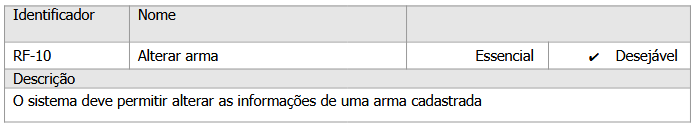
\includegraphics[scale=0.9]{imagens/rf10.png}
    \label{tab:rf10}
    \legend{Fonte: Autor}
\end{table}

\begin{table}[h]
    \caption{Requisito Funcional 11}
    \centering
    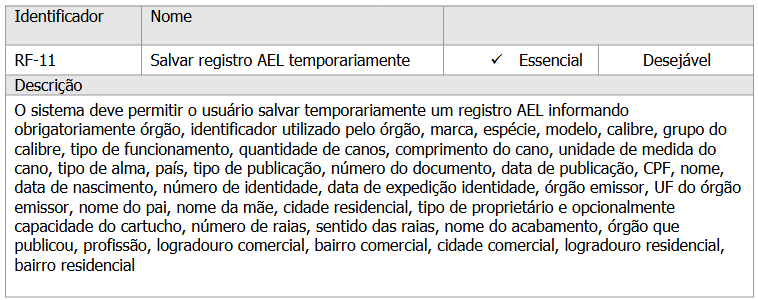
\includegraphics[scale=0.9]{imagens/rf11.png}
    \label{tab:rf11}
    \legend{Fonte: Autor}
\end{table}

\begin{table}[h]
    \caption{Requisito Funcional 12}
    \centering
    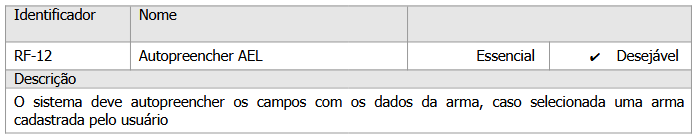
\includegraphics[scale=0.9]{imagens/rf12.png}
    \label{tab:rf12}
    \legend{Fonte: Autor}
\end{table}

\begin{table}[h]
    \caption{Requisito Funcional 13}
    \centering
    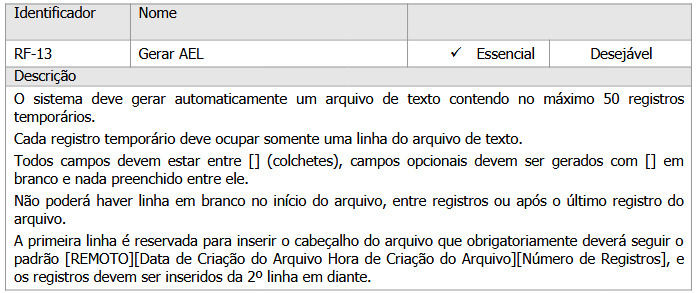
\includegraphics[scale=0.9]{imagens/rf13.png}
    \label{tab:rf13}
    \legend{Fonte: Autor}
\end{table}

\begin{table}[h]
    \caption{Requisito Funcional 14}
    \centering
    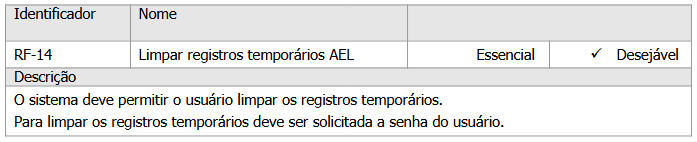
\includegraphics[scale=0.9]{imagens/rf14.png}
    \label{tab:rf14}
    \legend{Fonte: Autor}
\end{table}

\subsection{Requisitos Não Funcionais}
Na presente subseção, serão apresentados os requisitos não funcionais da aplicação, os quais descrevem as características globais do sistema, indo além das funcionalidades específicas.
Garantindo uma visão abrangente e integral.

\section*{sou um texto importante}
dasjdhnasjdksajk
% \begin{table}[h]
%     \caption{Requisito Não Funcional 1}
%     \centering
%     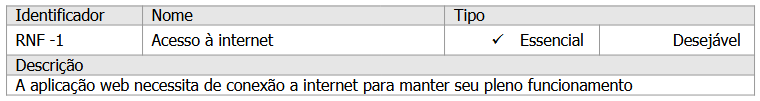
\includegraphics[scale=0.9]{imagens/rnf1.png}
%     \label{tab:rnf1}
%     \legend{Fonte: Autor}
% \end{table}

% \begin{table}[h]
%     \caption{Requisito Não Funcional 2}
%     \centering
%     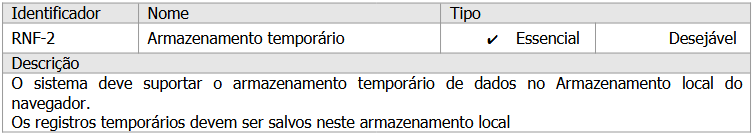
\includegraphics[scale=0.9]{imagens/rnf2.png}
%     \label{tab:rnf2}
%     \legend{Fonte: Autor}
% \end{table}

% \begin{table}[h]
%     \caption{Requisito Não Funcional 3}
%     \centering
%     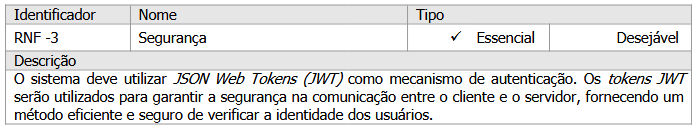
\includegraphics[scale=0.9]{imagens/rnf3.png}
%     \label{tab:rnf3}
%     \legend{Fonte: Autor}
% \end{table}

% \begin{table}[h]
%     \caption{Requisito Não Funcional 4}
%     \centering
%     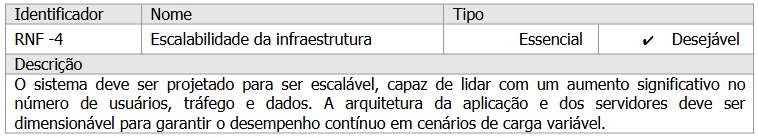
\includegraphics[scale=0.9]{imagens/rnf4.png}
%     \label{tab:rnf4}
%     \legend{Fonte: Autor}
% \end{table}

% \begin{table}[h]
%     \caption{Requisito Não Funcional 5}
%     \centering
%     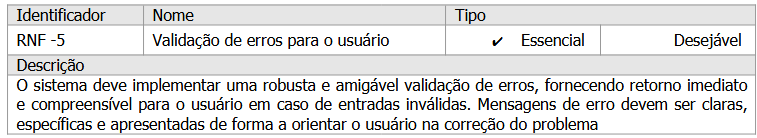
\includegraphics[scale=0.9]{imagens/rnf5.png}
%     \label{tab:rnf5}
%     \legend{Fonte: Autor}
% \end{table}
% % ---
% \section{Tabelas}
% % ---

% \index{tabelas}A \autoref{tab-nivinv} é um exemplo de tabela construída em
% \LaTeX.

% \begin{table}[htb]
% \ABNTEXfontereduzida
% \caption[Níveis de investigação]{Níveis de investigação.}
% \label{tab-nivinv}
% \begin{tabular}{p{2.6cm}|p{6.0cm}|p{2.25cm}|p{3.40cm}}
%   %\hline
%    \textbf{Nível de Investigação} & \textbf{Insumos}  & \textbf{Sistemas de Investigação}  & \textbf{Produtos}  \\
%     \hline
%     Meta-nível & Filosofia\index{filosofia} da Ciência  & Epistemologia &
%     Paradigma  \\
%     \hline
%     Nível do objeto & Paradigmas do metanível e evidências do nível inferior &
%     Ciência  & Teorias e modelos \\
%     \hline
%     Nível inferior & Modelos e métodos do nível do objeto e problemas do nível inferior & Prática & Solução de problemas  \\
%    % \hline
% \end{tabular}
% \legend{Fonte: \citeonline{van86}}
% \end{table}

% Já a \autoref{tabela-ibge} apresenta uma tabela criada conforme o padrão do
% \citeonline{ibge1993} requerido pelas normas da ABNT para documentos técnicos e
% acadêmicos.

% \begin{table}[htb]
% \IBGEtab{%
%   \caption{Um Exemplo de tabela alinhada que pode ser longa
%   ou curta, conforme padrão IBGE.}%
%   \label{tabela-ibge}
% }{%
%   \begin{tabular}{ccc}
%   \toprule
%    Nome & Nascimento & Documento \\
%   \midrule \midrule
%    Maria da Silva & 11/11/1111 & 111.111.111-11 \\
%   \midrule 
%    João Souza & 11/11/2111 & 211.111.111-11 \\
%   \midrule 
%    Laura Vicuña & 05/04/1891 & 3111.111.111-11 \\
%   \bottomrule
% \end{tabular}%
% }{%
%   \fonte{Produzido pelos autores.}%
%   \nota{Esta é uma nota, que diz que os dados são baseados na
%   regressão linear.}%
%   \nota[Anotações]{Uma anotação adicional, que pode ser seguida de várias
%   outras.}%
%   }
% \end{table}
% ---


